\problemname{Teiknum Krossa}

Tómas litli elskar að teikna krossa á rúðustrikuð blöð. Hann teiknar oft marga
krossa á hvert blað, en hver kross lítur út eins og á eftirfarandi mynd:

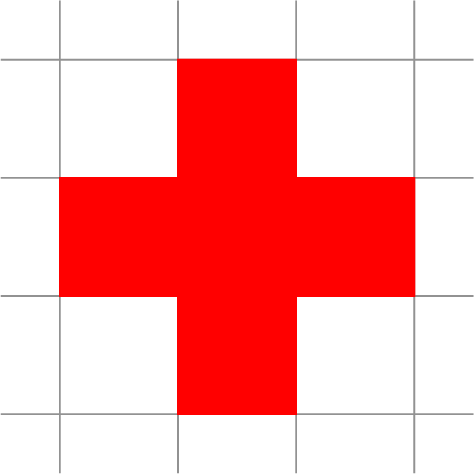
\includegraphics[scale=0.4]{cross.png}

Hann teiknar aldrei kross yfir annan kross, en teiknar þá þó oft hlið við hlið
eins og sjá má á eftirfarandi mynd:

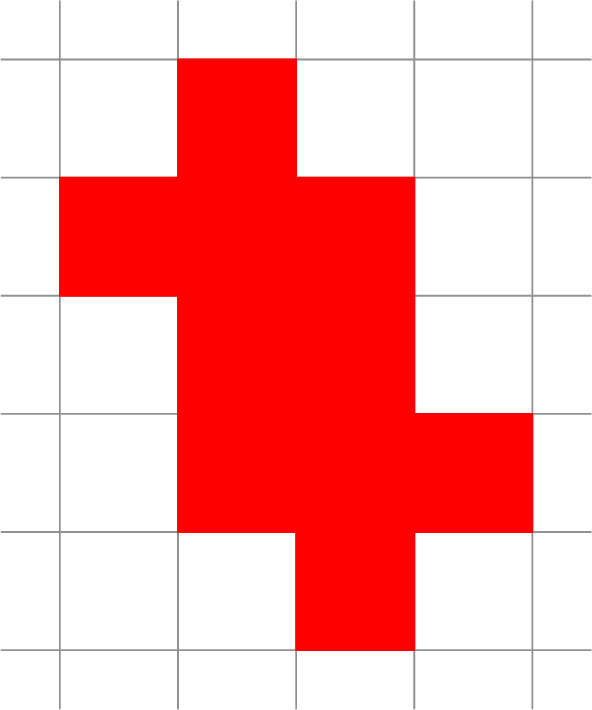
\includegraphics[scale=0.4]{two_crosses.png}

Tómas er búinn að teikna svona krossa á mörg blöð, og er byrjaður að blanda
þeim saman við aðrar teikningar. Núna ætlar hann að taka til, og flokka
teikningarnar sínar. Nú biður hann þig um hjálp. Hann lætur þig fá rúðustrikað
blað með teikningu á og vill fá að vita hvort það sé hugsanlegt að það séu
eingöngu krossar á teikningunni.

Á fyrstu línu inntaksins er heiltalan $1 \leq n \leq 100$. Þar eftir fylgja $n$
línur, hver með $n$ stafi, sem lýsir rúðustrikaða blaðinu. Fylltur kassi (eða
rúða) á blaðinu er táknuð með stafnum \texttt{"\#"}, en tómur kassi
er táknaður með \texttt{"."}. Engir aðrir stafir koma fyrir í
lýsingunni. Úttak inniheldur \texttt{"Jebb"} ef hugsanlegt er að
eingöngu krossar séu í teikningunni, en \texttt{"Neibb"} annars.

